\documentclass[UTF8,printbox,a4paper]{BHCexam}
\begin{document}
\biaoti{~$2013 - 2014$~学年第二学期期中考试试卷}
\fubiaoti{高二数学}
\maketitle
\notice

\begin{questions}
\xuanze
\question 在复平面内,复数~$1+i$~记作~对应的点位于\stk{A}.\\
\onech{第一象限}{第二象限}{第三象限}{第四象限}

\question 若输入~$a=3,b=4$~,则通过下列程序框图输出结果是\stk{C}.\\
\begin{figure}[htp]
  \centering
  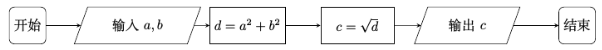
\includegraphics[scale=0.7]{liuchengtu.png}
\end{figure}
\onech{$\pm 5$}{$-5$}{$5$}{$4$}

\question 下列四个关系中,正确的是\stk{D}.\\
\onech{$\varnothing \in \{a \}$}{$a \notin \{a\}$}{$\{a \} \in \{a,b\}$}{$a\in \{a,b\}$}

\question 设~$P=\{x|x>0 \},Q=\{x|-1<x<2 \}$~,那么~$P\cap Q=$~\stk{B}.\\
\twoch{~$\{x|x>0$~或~$x\leq -1 \}$~}{~$\{x|0<x<2 \}$~}{~$\{x|x>0$~且~$x\leq -1 \}$~}{~$\{x|x\geq 2 \}$~}
\question 下列各组函数中,表示同一函数的是\stk{B}.\\
\twoch{$y=1,y=\dfrac{x}{x}$}{$y=x,y=\sqrt[3]{x^3}$}{$y=\lg x^2,y=2\lg x$}{$y=\abs{x},y=(\sqrt{x})^2$}
\question 若~$a=0.3 ^2,b=\log_2 0.3,c=2^{0.3}$~,则~$a,b,c$~的大小关系是\stk{C}.\\
\onech{$a<c<b$}{$a<b<c$}{$b<a<c$}{$b<c<a$}
\question 已知函数~$f(x)=x^2+x+1,x\in [0,\dfrac{3}{2}]$~的最值情况为\stk{C}.\\
\twoch{有最大值~$\dfrac{3}{4}$~,但无最小值}{有最小值~$\dfrac{3}{4}$~,有最大值~$1$~}{有最小值~$1$~,有最大值~$\dfrac{19}{4}$~}{无最大值,也无最小值}
\question 函数~$y=\sqrt{\log_ \frac{1}{2}{(2x-1)}}$~的定义域为\stk{C}.\\
\onech{$(\dfrac{1}{2},+\infty)$}{$[1,+\infty)$}{$(\dfrac{1}{2},1]$}{$(-\infty,1)$}
\question 已知~$f(\dfrac{1}{x})=\dfrac{1}{1+x}$~,那么函数~$f(x)$~的解析式及定义域正确的是\stk{B}.\\
\twoch{$f(x)=\dfrac{x}{1+x}(x\neq -1)$}{$f(x)=\dfrac{x}{1+x}(x\neq -1$且$x\neq 0)$}{$f(x)=\dfrac{1}{1+x}$}{$f(x)=1+x$}
\question 设$f(x)$是奇函数,且当~$x\in (0,+\infty)$~时,~$f(x)=x(1+x)$~,则当~$x\in (-\infty,0)$~时,~$f(x)$~等于\stk{C}.\\
\onech{$x(1+x)$}{$-x(1+x)$}{$x(1-x)$}{$-x(1-x)$}

\tiankong
\question  已知函数~$f(x)=\Bigg \{\begin{aligned} 
&\log_2 x ~~  (x>0) \\ 
&3^x ~~  (x\leq 0)  
\end{aligned}$~,则~$f[f(\dfrac{1}{4})]$~的值是~\stk{$\dfrac{1}{9}$}.

\question 已知幂函数~$y=f(x)$~的图象过点~$(2,\sqrt{2})$~,则~$f(9)=$~\stk{$3$}.

\question 当~$\dfrac{2}{3} <m<1$~时,复数~$m(3+i)-(2+i)$~在复平面内对应的点位于\stk{第四象限}.
\question 若有一组数据的总偏差平方和为~$100$~,相关指数~$R^2$~为~$0.8$~,则残差平方和为\stk{$40$}.


\jianda
\question 计算题
\begin{parts}
\part[6] $(0.25)^\frac{1}{2}-[-2\times (\dfrac{3}{7})^0]^2\times [(-2)^3]^\frac{4}{3}+(\sqrt{2}-1)^{-1}-2^{\frac{1}{2}}$;
\part[6] $(\lg5)^2+\lg2 \times \lg50$.
\end{parts}
\vspace{6cm}	
%\begin{solution}
%\begin{parts}
%\part $z=3+4\textbf{i}$
%\part $\abs{z-w}\in[4,6]$
%\end{parts}
%\end{solution}
%\clearpage

\question[12] 画出函数~$f(x)=x^2-\abs{2x-1}$~的图象,指出~$f(x)$~的单调区间.

\vspace{6cm}	
%\clearpage

\question 已知函数~$f(x)=4-x^2$
\begin{parts}
\part[7] 试判断函数~$f(x)$~的奇偶性,并证明函数~$f(x)$~在~$[0,+\infty)$~是减函数;
\part[6] 解不等式~$f(x)\geq 3x$~.
\end{parts}
\vspace{8cm}	
%\clearpage

\question 已知集合~$A=\{x\inR |ax^2-3x-4=0 \}$~.
\begin{parts}
\part[7] 若~$A$~中有两个元素,求实数~$a$~的取值范围;
\part[6] 若~$A$~中至多有一个元素,求实数~$a$~的取值范围.
\end{parts}

\end{questions}
\end{document}
